\chapter{État de l'art des techniques}
\chaptermark{Techniques}
\minitoc
\newpage
 
\section{Introduction}
Notre état de l'art va donc tourner autour des algorithmes d'apprentissage supervisé qui peuvent nous permettre de faire de la prédiction de panne encore appelée maintenance prédictive. Nous avons trouvé deux articles qui traitent de ce genre de problématique.

\section{Comparaison entre Random Forest et Decision Tree}
Nous allons utiliser cet article [2] dans lequel ont été comparés entre eux les efficacités des algorithmes de Random Forest et Arbre de Décision. Pour faire ce test, dans l'article on a utilisé les données du cancer du sein se trouvant dans la base de données  UCI Machine Learning repository [3]. 
\begin{figure}[h]
\begin{center}
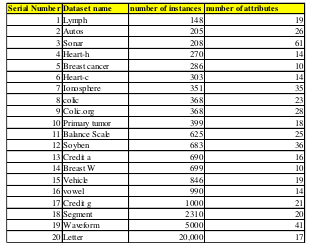
\includegraphics[scale=1.2]{dataset.png}
\caption[Caractéristiques et détails sur le jeu de données]{Caractéristiques et détails sur le jeu de données}
\label{monlabel}
\end{center}
\end{figure}

\newpage
\begin{figure}[h]
\begin{center}
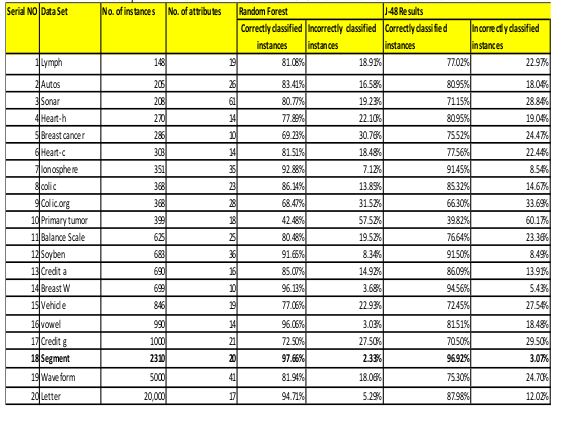
\includegraphics[scale=0.80]{validation_dataset_RF_DT.png}
\caption[Comparaison du F1 score  de Random Forest (J48) et Arbre de décision sur 20 jeu de données]{Comparaison du F1 score d'apprentissage de Random Forest (J48) et Arbre de décision sur 20 jeu de données}
\label{monlabel}
\end{center}
\end{figure}
Dans les résultats présents dans le tableau ci-dessous, nous remarquons que dans les deux cas les algorithmes ont un pourcentage d'apprentissage assez élevé. Si nous comparons les scores des deux algorithmes d'apprentissage nous remarquons que le random forest donne de meilleurs résultats pour des grands ensemble de données c'est à dire des données avec des grands nombre d'instance alors que les Arbres de décision sont meilleurs sur des petits jeux de données avec de nombre d'instance assez faible. Les résultats des tests sur les données du cancer du sein  montrent que lorsque le nombre d'instance est passé de 286 à 699, le nombre des instances correctement classés est passé de 69,23\% à 29,13\% pour les forêts aléatoires.
\newpage
\begin{figure}[h]
\begin{center}
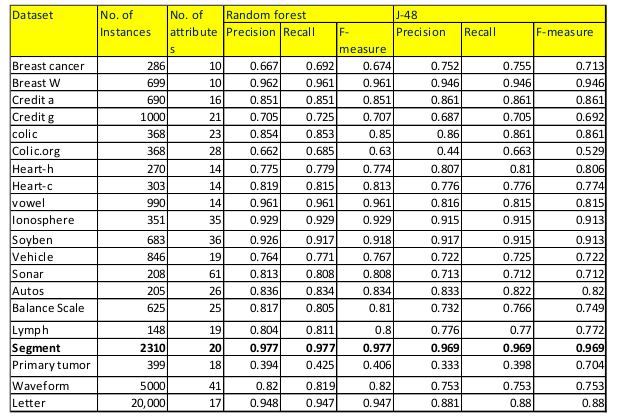
\includegraphics[scale=0.70]{ROC_Comparaison.png} 
\caption[Comparaison des scores Precision, Recall et F-measure de Random Forest (J48) et Arbre de décision sur 20 jeu de données]{Comparaison des scores Precision, Recall et F-measure de Random Forest (J48) et Arbre de décision sur 20 jeu de données}
\label{monlabel}
\end{center}
\end{figure}
Le tableau ci-dessous  présente des valeurs de validation des algorithmes dans le tableau pour
Random Forest et Arbre de décision pour les 20 jeux de données. Dans la  table, on peut voir que pour le même ensemble de données avec une plus grande nombre d'instances, c'est-à-dire lorsque le nombre d'instances
passe de 286 à 699 tout en conservant les attributs constante Precision augmente de 0,667 à 0,962, F-measure
de 0,674 à 0,961 et Recall de 0,692 à 0.961 pour le classificateur Random Forest. De même pour le
J48, Precision est passée de 0,752 à 0,946, F-measure de 0,713 à 0,946 et Recall de 0,755 à
0.946. La valeur de précision la plus élevée obtenue est pour le Random Forest, c'est-à-dire 0,977 pour l'ensemble de données.
D'après les résultats, on peut conclure que le Random Forest atteint des performances de classification accrues et donne des résultats exacts et précis dans les cas de grand nombre d'instances. Ces scénarios couvrent également les
problème de valeurs manquantes dans les jeux de données, il surmonte également le problème de sur-ajustement
généré en raison de valeurs manquantes dans les ensembles de données. Par conséquent, pour les problèmes de classification, si l'on doit choisir un classificateur parmi l'ensemble des classificateurs basés sur l'arbre, il est fortement recommandé d'utiliser le Random Forest en toute confiance pour divers problèmes de classification.


\section{Prédiction de pannes DSL par mesure passive sur des passerelles domestiques}
Dans cet article [1], l'objectif visé est de faire de la détection proactive des problèmes de ligne DSL. Pour ce faire les données qui ont été exploitées, sont des données collectées des informations liées au DSL à partir d'un ensemble de réseaux dosmestiques une période de deux années dont l'ensemble cumulative comprend 98 maisons d'essai sur une duréee cumulée de cette expérience d'essai est de 35455 jours. 

\begin{itemize}[label=\textbullet, font=\LARGE \color{black}]
\item Expérimentations
\newline
Les compteurs CNT comptent le nombre d'évènements dans une période d'interrogation (une minute). Les tarifs et les valeurs de bruit sont les valeurs actuelles telles que récupérées par le client au moment de la collecte.
\begin{figure}[h]
\begin{center}
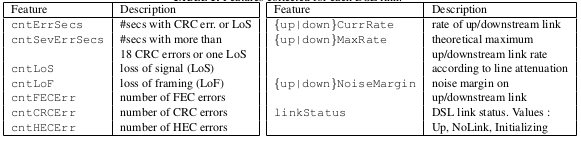
\includegraphics[scale=0.70]{Features.png}
\caption[Caractéristiques collectées pour chaque lien DSL]{Caractéristiques collectées pour chaque lien DSL}
\label{monlabel}
\end{center}
\end{figure}

\item Evaluations et résultats
\newline
\begin{figure}[h]
\begin{center}
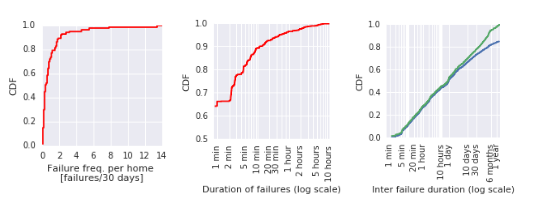
\includegraphics[scale=0.80]{Feature_2.png}
\caption[Caractéristiques de défaillance]{Caractéristiques de défaillance}
\label{monlabel}
\end{center}
\end{figure}
Les algorithmes qui ont été appliqués sur le jeu de données sont entre autres Random Forest, Naive Bayésien, AdaBoost, Décision Tree.
Ci-dessous une figure comparative des résultats obtenus.
\begin{figure}[h]
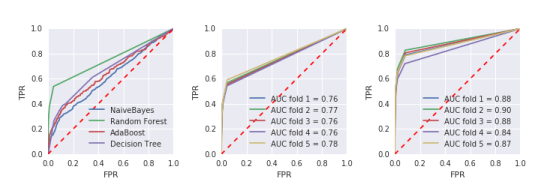
\includegraphics[scale=0.80]{Evaluation.png}
\caption[Evaluation et choix du meilleur modèle]{Evaluation et choix du meilleur modèle}
\label{monlabel}
\end{figure}
Au vue de ces expérimentations, nous pouvons conclure que le Random Forest nous permet d'avoir les meilleurs résultats.

\end{itemize}

\section{Conclusion}
En somme ces techniques d'apprentissage supervisé nous permettront de faire de la maintenance prédictive.